\documentclass[12pt]{article}
\usepackage[margin=1in]{geometry} 
\usepackage{amsmath,amsthm,amssymb,amsfonts}
\usepackage{graphicx}
 
\newcommand{\N}{\mathbb{N}}
\newcommand{\Z}{\mathbb{Z}}
 
\newenvironment{problem}[2][Problem]{\begin{trivlist}
\item[\hskip \labelsep {\bfseries #1}\hskip \labelsep {\bfseries #2.}]}{\end{trivlist}}
 
\begin{document}
 
%Good resources for looking up how to do stuff:
%Binary operators: http://www.access2science.com/latex/Binary.html
%General help: http://en.wikibooks.org/wiki/LaTeX/Mathematics
%Or just Google stuff
 
\title{Homework 3}
\author{Tanner Kvarfordt - A02052217}
\maketitle
 
\begin{problem}{1}
Prove that the following game must have a winner. Place 6 dots equally spaced on a circle on a piece of paper. Player A has a red marker and Player B has a blue marker. Players take turns connecting pairs of dots with line segments using their respective colored markers, only one line segment between any two dots (therefore at most 15 line segments will be drawn). The winner is the first to connect three dots mutually with their respective color, that is, the first to create a monochromatic "triangle" in their marker's color.
\end{problem}
 
\begin{proof}
As stated in the problem, there is a maximum of fifteen line segments that may be drawn, five for each pair of dots. For the sake of proving that there is always a winner of the game, we will assume for this proof that the game is played so that all fifteen possible line segments are always drawn. It is logical after all that if less than the possible fifteen are drawn, then there was a winner. So the case where all fifteen line segments must be drawn is the only case that concerns this proof. Now, because any given dot must have five line segments emanating from it for the case we are considering, and because each player draws one line segment per turn, it is clear that, at a minimum, three of the five line segments emanating from any given dot will be the same color. More are possible, but three is the minimum. Consider a dot where this is the case, a dot that has three line segments of color $c_1$ and two line segments of color $c_2$ emanating from it. Disregard, for the moment, the destinations of the two $c_2$ line segments and consider only the destinations of the three $c_1$ line segments. We know that these destination dots also must have all five line segments emanating from them, and that, for each one, at least three of them will be the same color. We also know that they must be connected to each other. Now, because all three have a connection to the original dot, and because that connection is the same color for all three ($c_1$ in this case), if a line segment with color $c_1$ is used to connect any of those three dots, a monochromatic triangle is drawn and the game has a winner. If the opposite color, $c_2$, manages to block all three of these winning moves, then a monochromatic triangle of $c_2$ is drawn, and the game has a winner. Therefore, it is clear that the game must always have a winner. Refer to figure 1 for visual aide for this proof. I apologize for my atrocious LaTeX image skills. I am still learning. :)
\begin{figure}[ht!]
\centering
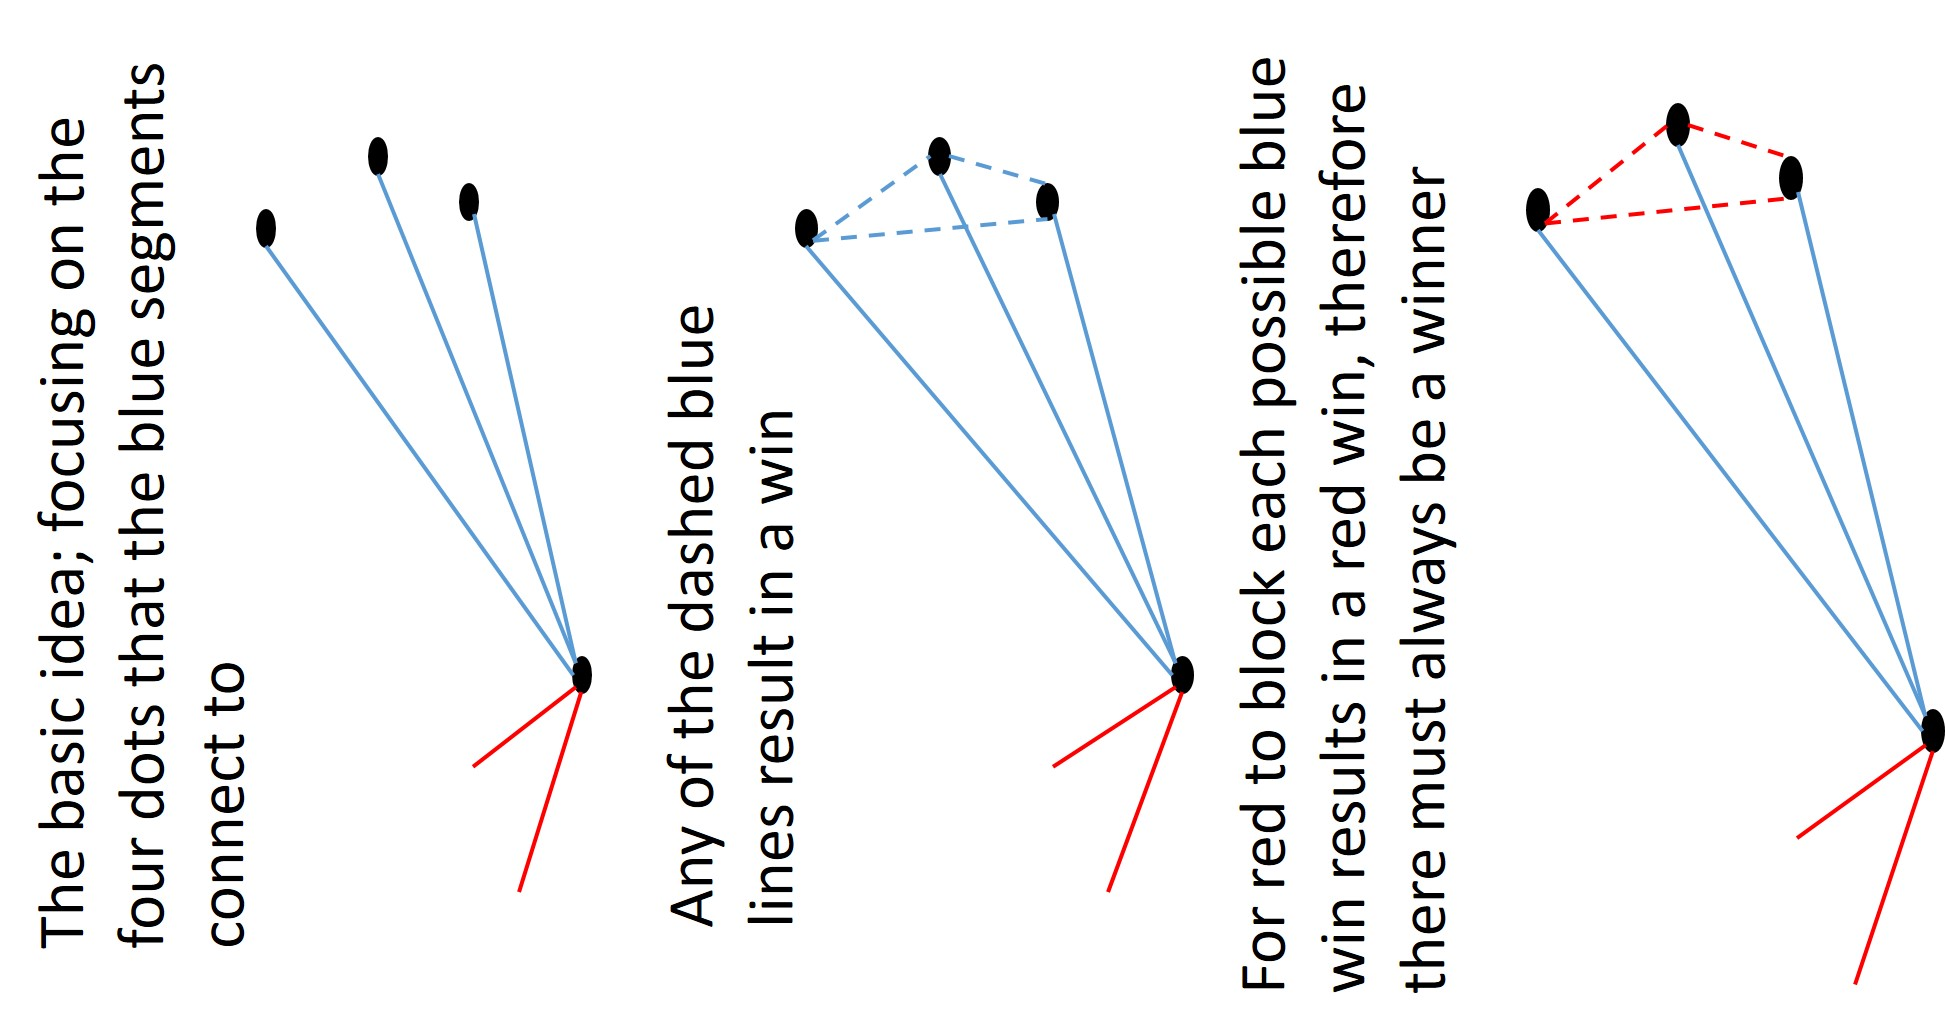
\includegraphics[width=115mm]{Capture}
\caption{Dot Game Diagram}
\end{figure}
\end{proof}
\newpage
\begin{problem}{2}
Consider the following sets: $\mathbb{N}$, the set of non-negative integers; $\mathbb{E}$, the set of even integers (negative ones too); $\mathbb{Z}$, the set of integers.
\begin{description}
\item \textbf{(a)} Please prove that each of the sets $\mathbb{N}$, $\mathbb{E}$, and $\mathbb{Z}$ are infinite.
\end{description}
\end{problem}

\begin{proof}
As stated in Dr. Brown's Meeting Notes Seven, a set $A$ is infinite if there is a bijection from a proper subset of itself (we'll call this subset $B$) to itself, or vice-versa. A bijection, as also defined by Dr. Brown, is a function between the elements of two sets that is both one-to-one and onto. A function $f$ is one-to-one if $f(a_1) = f(a_2) \implies a_1 = a_2$, for $a_1,a_2 \in A$. The function $f$ is onto if, for every $b \in B$, there exists an $a \in A$ such that $f(a) = b$. For use in the proofs below, define the set $\mathbb{E}^+$ to be the set of non-negative even integers. The proofs that the sets $\mathbb{N}$, $\mathbb{E}$, and $\mathbb{Z}$ are infinite follow below:
\newline
\newline
\textit{Proving that $\mathbb{N}$ is infinite:} The set $\mathbb{E}^+$ is a proper subset of $\mathbb{N}$ and, I claim, the function $f:\mathbb{N} \rightarrow \mathbb{E}^+$ defined by $f(x)=2x$ for some $x \in\mathbb{N}$ is a bijection. To see that $f$ is onto, consider an element $b \in\mathbb{E}^+$, and an element $a \in\mathbb{N}$. Let $a=\frac{b}{2}$, then $f(a)=f(\frac{b}{2})=2(\frac{b}{2}) = b$. To see that $f$ is one-to-one, suppose $f(x_1)=f(x_2)$. Then $f(x_1)=2(x_1) = 2(x_2) = f(x_2)$, and so divide both sides of the equation by two to get $\frac{1}{2}2(x_1) = \frac{1}{2}2(x_2)$, then simplify the fractions to see that $x_1=x_2$. Therefore, since $f$ is a bijection from $\mathbb{N}$ to a proper subset of $\mathbb{N}$, $\mathbb{N}$ is infinite.
\newline
\newline
\textit{Proving that $\mathbb{E}$ is infinite:} To begin this proof, I will first define the set $\mathbb{E}^\# = \{q \in\mathbb{E}^\# : q=2(k+1)$ for some $k \in\mathbb{E}\}$. Please note that if the notation of a set to the power of the "\#" symbol actually means something in the mathematical world, then I disagree with that meaning vehemently and substitute my own - that meaning being, of course, that it is a convenient way to denote that $\mathbb{E}^\#$ is some sort of set governed by the definition I just provided. Moving on, I assert that $\mathbb{E}^\#$ is a proper subset of $\mathbb{E}$, the proof of which lies in the fact that, by definition, $q$ is an even number, but $q$ will never be $0$, or even $4$ for that matter. Therefore $\mathbb{E}^\#$ is a proper subset of $\mathbb{E}$. Now that that fact has been established, I claim that the function $f:\mathbb{E}\rightarrow \mathbb{E}^\#$ defined by  $f(x)=2(x+1)$ for some $x \in\mathbb{E}$ is a bijection. To see that $f$ is onto, consider an element $b \in\mathbb{E}^\#$, and an element $a \in\mathbb{E}$. Let $a = \frac{b}{2} - 1$, then $f(a)=f(\frac{b}{2}-1)=2(\frac{b}{2}-1+1)=b$. To see that $f$ is one-to-one, suppose $f(x_1)=f(x_2)$. Then $f(x_1)=2(x_1 + 1) = 2(x_2 + 1) = f(x_2)$. Divide both sides of the equation by two to get $x_1 +1 = x_2 + 1$, and then subtract one from both sides to see that $x_1 = x_2$. Therefore, since $f$ is a bijection from $\mathbb{E}$ to a proper subset of $\mathbb{E}$, $\mathbb{E}$ is infinite.
\newline
\newline
\textit{Proving that $\mathbb{Z}$ is infinite:} The set $\mathbb{E}$ is a proper subset of $\mathbb{Z}$, and I claim, the function $f:\mathbb{Z} \rightarrow \mathbb{E}$ defined by $f(x)=2x$ for some $x \in\mathbb{Z}$ is a bijection. To see that $f$ is onto, consider an element $b \in\mathbb{E}$, and an element $a \in\mathbb{Z}$. Let $a = \frac{b}{2}$, then $f(a)=f(\frac{b}{2})=2(\frac{b}{2}) = b$. To see that $f$ is one-to-one, suppose $f(x_1)=f(x_2)$. Then $f(x_1)=2(x_1) = 2(x_2) = f(x_2)$, and so divide both sides of the equation by two to get $\frac{1}{2}2(x_1) = \frac{1}{2}2(x_2)$, then simplify the fractions to see that $x_1=x_2$. Therefore, since $f$ is a bijection from $\mathbb{Z}$ to a proper subset of $\mathbb{Z}$, $\mathbb{Z}$ is infinite.
\end{proof}

\begin{description}
\item \textbf{(b)} Please prove that the sets $\mathbb{Z}$ and $\mathbb{E}$ have the same cardinality.
\end{description}

\begin{proof}
As defined in Dr. Brown's Meeting Notes Seven, two sets have the same cardinality if there is a bijection from one to the other. Because the sets we are dealing with here are $\mathbb{Z}$ and $\mathbb{E}$, this will be a rather short proof. I simply refer you to part \textbf{(a)} of this problem, where I prove that $\mathbb{Z}$ is infinite. There you will find proof that the function $f(x)=2x$ is a bijection from $\mathbb{Z}$ to $\mathbb{E}$, and therefore, the sets $\mathbb{Z}$ and $\mathbb{E}$ have the same cardinality. 
\end{proof}

\begin{problem}{3}
Please prove the open interval $(0,1) = \{x \in\mathbb{R} : 0 < x < 1\}$ does not have the same cardinality as $\mathbb{N}$.
\end{problem}
 
\begin{proof}
Proof would go here if I could figure out how to do this.
\end{proof}

\end{document}